%\documentclass[oneside, 11pt, a4paper]{article}
\documentclass[a4paper,11pt]{article}

%\usepackage{algorithmicx}
%\usepackage[linesnumbered,lined,boxed,commentsnumbered]{algorithm2e}
\usepackage[utf8]{inputenc}
\usepackage{algorithm}
\usepackage{algpseudocode}
\usepackage{graphicx} 
\usepackage{array}
\usepackage[table,xcdraw]{xcolor}
%\usepackage{subfigure}
\usepackage{url}
\usepackage{comment}
\usepackage{fancyhdr}
\usepackage{float}
\usepackage{multicol}
\usepackage{amsmath}
\usepackage{amssymb}
\usepackage{pifont}
%\usepackage{cite}
\usepackage{multirow}
\usepackage{fancybox}
\usepackage{paralist}
\usepackage{setspace}  
\usepackage{amssymb}
\usepackage{textcomp}
\usepackage{fontspec}
\usepackage{caption}
\newcounter{tablerow}
\usepackage{diagbox}
\usepackage{chngcntr}
\usepackage{relsize}
\usepackage{capt-of}
\usepackage{booktabs}
\usepackage{varwidth}
\usepackage{lipsum}
\newsavebox\tmpbox
\usepackage{amssymb}
\usepackage{endnotes}
\usepackage{lipsum}
\usepackage[hyperfootnotes=true, colorlinks=true]{hyperref}
 \hypersetup{
	colorlinks=true,
	linkcolor=black,
	filecolor=black,
	citecolor = black,      
	urlcolor=cyan,
}
\usepackage{hyperendnotes}
\usepackage{cleveref}


\newcommand{\crefrangeconjunction}{--}
\crefformat{tablerow}{#2#1#3}
\crefmultiformat{tablerow}{#2#1#3}%
{ و~#2#1#3}%
{, #2#1#3}%
{ و~#2#1#3}



%\usepackage[style=ieee]{biblatex}
%\bibliography{resources}

%\doublespacing


%\usepackage[top=29mm, bottom=29mm, left=19mm, right=19mm]{geometry}
\usepackage[top=1.1in, bottom=1.1in, left=0.75in, right=0.75in]{geometry}

\usepackage{xepersian}


\newtheorem{definition}{تعريف}
\newtheorem{theorem}{قضيه}
\defpersianfont\keywordsfont[Scale=1.0]{B Nazanin}
\defpersianfont\titlefont[Scale=1.1]{B Nazanin}
\defpersianfont\titlelatinfont[Scale=1.0]{Times New Roman}
\defpersianfont\secondtitlefont[Scale=1.0]{B Nazanin} %1.4
\defpersianfont\secondtitlelatinfont[Scale=0.9]{Times New Roman}

\settextfont[Scale=1.0]{B Nazanin}
\setlatintextfont[Scale=0.9]{Times New Roman}
%\setdigitfont[Scale=1]{XB Niloofar}
%\setromantextfont[Scale=1.2]{XB Niloofar} 
\defpersianfont\sectionsfont[Scale=1.0]{B Nazanin}
\defpersianfont\captionsfont[Scale=1.0]{B Nazanin}



\usepackage{sectsty}
\allsectionsfont{\sectionsfont}


\linespread{1} %line space
%\setstretch{1}
\small
\setlength{\parindent}{5pt} %The indent of the paragraph first line
\setlength{\parskip}{5pt} %Befor paragraph space

\setlength{\columnsep}{6mm}
%\let\footnote=\endnote
\renewcommand{\notesname}{واژه‌نامه‌}
\newcommand{\myitem}{\settextfont[Scale=0.9]{XB Niloofar}\item[\textbullet]\settextfont[Scale=1.0]{B Nazanin}}

\renewcommand\refname{\rl{ منابع و مراجع}}

\def\InE{\begingroup\beginL\latinfont}
\def\EnE{\endL\endgroup} 
\def\InF{\begingroup\beginR\persianfont}
\def\EnF{\endR\endgroup}
\newcommand{\IE}[1]{\lr{#1}}
\newcommand{\IP}[1]{\rl{#1}} 
\newcommand{\IF}[1]{\rl{#1}}
\definecolor{ao(english)}{rgb}{0.0, 0.5, 0.0}
\newcommand{\cmark}{\textcolor{ao(english)}{\ding{52}}}%
\newcommand{\xmark}{\textcolor{red}{\ding{56}}}%

\def\persiandash{\rl{-}}

\newcommand{\efootnote}[1]{\endnote{\lr{#1}}}
%\newcommand{\ecfootnote}[1]{}

\let\oldemph=\emph
\renewcommand{\emph}[1]{''\oldemph{#1}``}

\let\oldcaption=\caption
%\renewcommand{\caption}[1]{{\bf \captionsfont}}
\captionsetup[figure]{labelfont={bf},textfont={bf},labelsep = colon,font=small}
\captionsetup[table]{labelfont={bf},textfont={bf},labelsep = colon,font=small}
%\renewcommand{\caption}[1]{{\captionsfont -\arabic{section}\oldcaption{}}}
\counterwithin{figure}{section}
\counterwithin{table}{section}
\renewcommand{\thefigure}{\arabic{section}-\arabic{figure}}
\renewcommand{\thetable}{\arabic{section}-\arabic{table}}





%\renewcommand{\thechapter}{\tartibi{chapter}}
\renewcommand{\thesection}{\arabic{section}}
\renewcommand{\thesubsection}{\arabic{section}-\arabic{subsection}}
\renewcommand{\thesubsubsection}{\arabic{section}-\arabic{subsection}-\arabic{subsubsection}}

\newcommand{\authormajor}{معماری کامپیوتر} %گروه
\newcommand{\thesistitlepersian}{مدیریت دما در سامانه‌های بحرانی-مختلط چندهسته‌ای تحمل‌پذیر اشکال}%عنوان فارسی
\newcommand{\thesistitlelatin}{Thermal Management in Fault-Tolerant Mixed-Criticality Multicore Systems}%عنوان انگلیسی
\newcommand{\authorname}{پوریا گوهری}%نام و نام‌خانوادگی
\newcommand{\studentid}{9700000}%شماره دانشجویی


\newcommand{\advisorprofname}{دکتر شاهین حسابی} %persian:   استاد راهنما
\newcommand{\examinerprofname}{دکتر علیرضا اجلالی} %persian:   استاد ممتحن داخلي يا استاد مشاور

\renewcommand{\maketitle}{
\begin{titlepage}
\linespread{1.6} %line space

%\thispagestyle{fancy}

\begin{center}
\vspace*{-1cm}

\includegraphics[width=1.4in]{img/SharifLogo}\\[0.0cm]

\textbf{\titlefont
دانشگاه صنعتي شريف
\\
دانشکده مهندسي کامپيوتر
\\
سمينار کارشناسي ارشد گرايش
\authormajor
\\ [1.7cm]
}

\linespread{1.6} %line space

%\textbf{\titlefont
\settextfont[Scale=1.4]{B Nazanin}{\setlatintextfont[Scale=1.2]{Times New Roman} 
\textbf{
عنوان:
\\
\thesistitlepersian
\\
\lr{\thesistitlelatin}
\\ [2.0cm]
}
}
\linespread{1.6} %line space

\settextfont[Scale=1.4]{B Nazanin}{\setlatintextfont[Scale=1.2]{Times New Roman} 
	\textbf{
نگارش:
\\
\authorname
\\
\studentid
\\ [1.1cm]
استاد راهنما:
\\
\advisorprofname
\\ [1.0cm]
استاد ممتحن داخلي:
\\
\examinerprofname
\\ [4.0cm]
}
}

{\titlefont \textbf{
بهمن 98}
}\\[0.5cm]

\end{center}

\end{titlepage}
\setcounter{page}{1}
}


\begin{document} 
\maketitle %صفحه‌ی ابتدایی

\renewcommand*\thesection{\arabic{section}}
\textbf{\large{چکیده:}}
\label{sec:abstract}
لورم ایپسوم متن ساختگی با تولید سادگی نامفهوم از صنعت چاپ و با استفاده از طراحان گرافیک است. چاپگرها و متون بلکه روزنامه و مجله در ستون و سطرآنچنان که لازم است و برای شرایط فعلی تکنولوژی مورد نیاز و کاربردهای متنوع با هدف بهبود ابزارهای کاربردی می باشد. کتابهای زیادی در شصت و سه درصد گذشته، حال و آینده شناخت فراوان جامعه و متخصصان را می طلبد تا با نرم افزارها شناخت بیشتری را برای طراحان رایانه ای علی الخصوص طراحان خلاقی و فرهنگ پیشرو در زبان فارسی ایجاد کرد. در این صورت می توان امید داشت که تمام و دشواری موجود در ارائه راهکارها و شرایط سخت تایپ به پایان رسد وزمان مورد نیاز شامل حروفچینی دستاوردهای اصلی و جوابگوی سوالات پیوسته اهل دنیای موجود طراحی اساسا مورد استفاده قرار گیرد.


\noindent\keywordsfont\textbf{واژه‌های کلیدی:}
سامانه‌های بحرانی-مختلط، بسترهای چندهسته‌ای، تحمل‌پذیری اشکال، مدیریت دما

\section{مقدمه}
\label{sec:introduction}
لورم ایپسوم متن ساختگی با تولید سادگی نامفهوم از صنعت چاپ و با استفاده از طراحان گرافیک است. چاپگرها و متون بلکه روزنامه و مجله در ستون و سطرآنچنان که لازم است و برای شرایط فعلی تکنولوژی مورد نیاز و کاربردهای متنوع با هدف بهبود ابزارهای کاربردی می باشد. کتابهای زیادی در شصت و سه درصد گذشته، حال و آینده شناخت فراوان جامعه و متخصصان را می طلبد تا با نرم افزارها شناخت بیشتری را برای طراحان رایانه ای علی الخصوص طراحان خلاقی و فرهنگ پیشرو در زبان فارسی ایجاد کرد. در این صورت می توان امید داشت که تمام و دشواری موجود در ارائه راهکارها و شرایط سخت تایپ به پایان رسد وزمان مورد نیاز شامل حروفچینی دستاوردهای اصلی و جوابگوی سوالات پیوسته اهل دنیای موجود طراحی اساسا مورد استفاده قرار گیرد.

لورم ایپسوم متن ساختگی با تولید سادگی نامفهوم از صنعت چاپ و با استفاده از طراحان گرافیک است. چاپگرها و متون بلکه روزنامه و مجله در ستون و سطرآنچنان که لازم است و برای شرایط فعلی تکنولوژی مورد نیاز و کاربردهای متنوع با هدف بهبود ابزارهای کاربردی می باشد. کتابهای زیادی در شصت و سه درصد گذشته، حال و آینده شناخت فراوان جامعه و متخصصان را می طلبد تا با نرم افزارها شناخت بیشتری را برای طراحان رایانه ای علی الخصوص طراحان خلاقی و فرهنگ پیشرو در زبان فارسی ایجاد کرد. در این صورت می توان امید داشت که تمام و دشواری موجود در ارائه راهکارها و شرایط سخت تایپ به پایان رسد وزمان مورد نیاز شامل حروفچینی دستاوردهای اصلی و جوابگوی سوالات پیوسته اهل دنیای موجود طراحی اساسا مورد استفاده قرار گیرد.

\section{بررسی کارهای مرتبط پیشین}
\label{sec:survey}
تمرکز اصلی این پژوهش بر ارائه‌ی روش زمان‌بندی آگاه از دمای سطح تراشه و قابلیت اطمینان در سامانه‌های بحرانی-مختلط چند هسته‌ای همگن است. با توجه به آنکه سامانه‌های نهفته‌ی بحرانی-مختلط نوع ارتقاء یافته‌ای از سامانه‌های نهفته‌ی بحرانی-ایمن هستند\cite{Baruah2012b}، در این بخش سعی می‌شود به بررسی برخی کارهای مرتبط با این پژوهش و سامانه‌های بحرانی-مختلط در حوزه‌ی سامانه‌های بحرانی-ایمن نیز پرداخته شود. به همین منظور در ابتدا به بررسی کارهای پیشین در حوزه‌ی نگاشت و زمان‌بندی وظایف در سامانه‌های بحرانی-مختلط پرداخته می‌شود سپس به بررسی کار‌های پیشین در حوزه‌ی تحمل‌پذیری اشکال در سامانه‌های بحرانی-ایمن و بحرانی-مختلط پرداخته می‌شود و در انتها به بررسی پژوهش‌های حوزه‌ی مدیریت دما و سقف توان پرداخته می‌شود.

\subsection{نگاشت و زمان‌بندی وظایف در سامانه‌های بحرانی-مختلط}

\subsection{تحمل‌پذیری اشکال در سامانه‌های بحرانی-مختلط}

\subsection{مدیریت سقف توان مصرفی و حداکثر دمای سطح تراشه}
\begin{table}[b!]
\caption{جمع‌بندی و مقایسه روش‌های پیشین }
	\centering
\begin{tabular}{||c|c|c|c|c|c||}
	\hline
	روش                                                                              & بستر        & مدیریت دما/سقف توان & مدل سامانه& تحمل‌پذیری اشکال    & مدل وظایف         \\ \hline
	\cite{Baruah2008}\cite{Vestal2007}\cite{Baruah2015}\cite{Ekberg2014}             & تک‌هسته‌ای  & \xmark              & بحرانی-مختلط                                                                       & \xmark                  & پراکنده      \\ \hline
	\cite{Su2013}                                                                    & تک‌هسته‌ای  & \xmark              & بحرانی-مختلط                                                                      & \xmark                  & متناوب            \\ \hline
	\cite{Li2012}                                                                    & چند‌هسته‌ای & \xmark              &بحرانی-مختلط                                                                      & \xmark                  & پراکنده     \\ \hline
		روش پیشنهادی                                                                     & چندهسته‌ای  & \cmark              & بحرانی-مختلط                                                                        & افزونگی چندپیمانه‌ای & گراف-متناوب              \\ \hline
\end{tabular}
\label{tab:survey}
\end{table}




 

\section{راهکار پیشنهادی}
\label{sec:solution}
لورم ایپسوم متن ساختگی با تولید سادگی نامفهوم از صنعت چاپ و با استفاده از طراحان گرافیک است. چاپگرها و متون بلکه روزنامه و مجله در ستون و سطرآنچنان که لازم است و برای شرایط فعلی تکنولوژی مورد نیاز و کاربردهای متنوع با هدف بهبود ابزارهای کاربردی می باشد. کتابهای زیادی در شصت و سه درصد گذشته، حال و آینده شناخت فراوان جامعه و متخصصان را می طلبد تا با نرم افزارها شناخت بیشتری را برای طراحان رایانه ای علی الخصوص طراحان خلاقی و فرهنگ پیشرو در زبان فارسی ایجاد کرد. در این صورت می توان امید داشت که تمام و دشواری موجود در ارائه راهکارها و شرایط سخت تایپ به پایان رسد وزمان مورد نیاز شامل حروفچینی دستاوردهای اصلی و جوابگوی سوالات پیوسته اهل دنیای موجود طراحی اساسا مورد استفاده قرار گیرد.

لورم ایپسوم متن ساختگی با تولید سادگی نامفهوم از صنعت چاپ و با استفاده از طراحان گرافیک است. چاپگرها و متون بلکه روزنامه و مجله در ستون و سطرآنچنان که لازم است و برای شرایط فعلی تکنولوژی مورد نیاز و کاربردهای متنوع با هدف بهبود ابزارهای کاربردی می باشد. کتابهای زیادی در شصت و سه درصد گذشته، حال و آینده شناخت فراوان جامعه و متخصصان را می طلبد تا با نرم افزارها شناخت بیشتری را برای طراحان رایانه ای علی الخصوص طراحان خلاقی و فرهنگ پیشرو در زبان فارسی ایجاد کرد. در این صورت می توان امید داشت که تمام و دشواری موجود در ارائه راهکارها و شرایط سخت تایپ به پایان رسد وزمان مورد نیاز شامل حروفچینی دستاوردهای اصلی و جوابگوی سوالات پیوسته اهل دنیای موجود طراحی اساسا مورد استفاده قرار گیرد.

\subsection{مدل سامانه}
\textbf{مدل سخت‌افزار:}
در این پژوهش از بستر‌های چند‌ هسته‌ای با هسته‌های همگن استفاده می‌شود. در این مدل هر هسته به صورت مستقل می‌تواند ولتاژ و فرکانس خود را تغییر دهد. پردازنده‌ی اکسینوس4415\efootnote{Exynos4415} با چهار هسته‌ی مبتنی بر معماری آرم\efootnote{ARM} از خانواده‌ی \lr{Cortex-A9} نمونه‌ای از این بستر‌ها است. در مدل پیشنهادی هسته‌های پردازنده با مجموعه‌ی $\left \{p_1,p_2,p_3,...\right \}$ نشان داده‌می‌شود. در این پژوهش فرض می‌شود هر هسته قابلیت استفاده از سطوح مشخص ولتاژ و فرکانس را دارد. این ولتاژها و فرکانس‌ها به صورت مجموعه‌ی $\left \{(v_1,f_1),(v_2,f_2),(v_3,f_3),...\right \}$ نشان داده‌می‌شود. دمای فعال‌سازی سامانه پویای مدیریت گرمای پردازنده یا به عبارتی حداکثر دمای امن پردازنده با $T_{DTM}$ نشان داده‌می‌شود.\\
\begin{equation}
\label{eq:voltage_scale}
V_i=\rho _iV_{max} (\rho _{min}< \rho _i<\rho _{max}=1 )
\end{equation}
در رابطه‌ی فوق $\rho _i$ ضریب تغییر\efootnote{Scale} ولتاژ است.
\subsection{تأمین شرایط قابلیت اطمینان و تحمل‌پذیری اشکال}
همان‌گونه که گفته شد یکی از مهم‌ترین نیازمندی‌های سامانه‌های بحرانی-مختلط قابلیت اطمینان است. زمان‌بندی چندین نسخه از یک وظیفه بر روی هسته‌های مختلف احتمال اینکه حداقل یکی از آن‌ها به درستی اجرا شوند را بالا می‌برد و درنتیجه باعث بالا رفتن قابلیت اطمینان سامانه می‌شود\cite{Pathan2014}. به همین منظور در این پژوهش با توجه به سطح قابلیت اطمینان مورد نیاز و حداکثر تعداد اشکالی که باید بر روی یک وظیفه تحمل شود، تعداد افزونگی مورد نیاز برای سامانه تعیین می‌شود. در ادامه برای هر وظیفه سعی می‌شود ولتاژ و فرکانس اجرا به گونه‌ای انتخاب شود که قابلیت اطمینان مورد نیاز وظیفه حفظ شود. مطابق الگوریتم \ref{alg:minvf}  در ابتدا سطوح ولتاژ و فرکانس پردازنده را از کوچک به بزرگ مرتب می‌کنیم (خط 2). سپس برای هر زوج ولتاژ و فرکانس از کوچک به بزرگ قابلیت اطمینان وظیفه را مطابق رابطه‌ی \ref{eq:Rel_sum}  محاسبه‌ می‌کنیم. اگر قابلیت اطمینان  محاسبه شده بزرگ‌تر یا مساوی قابلیت اطمینان مورد نیاز باشد، زوج ولتاژ و فرکانس استفاده شده برای محاسبه‌ی قابلیت اطمینان، به عنوان کوچک‌ترین ولتاژ و فرکانسی که قابلیت اطمینان وظیفه را حفظ می‌کند برگردانده می‌شود (خطوط 3 تا 6). در صورتی که هیچ‌یک از سطوح ولتاژ و فرکانس پردازنده نتواند قابلیت اطمینان وظیفه را برآورده کند، زمان‌بندی سامانه غیر عملی\efootnote{Infeasible} است (خط 8).\\
	\begin{algorithm}[H]
		\caption{یافتن کوچک‌ترین ولتاژ و فرکانس برای برآورده کردن قابلیت اطمینان وظیفه}
		\label{alg:minvf}
		\latin
		\textbf{Input:} $\tau_i$: Task , $R_i$:Min. Reliability of $\tau_i$ ,$(v,f)$: processor voltage \& frequency levels  \\
		\textbf{Output:} $(v_i,f_i)$: min. voltage and frequency that keep reliability of $\tau_i$	
		\begin{algorithmic}[1]
			\Function{FindMinVF}{$\tau_i$,$R_i$,$(v,f)$}
			\State \textbf{Sort($(v,f)$)} \Comment{Sorting volt. \& freq. array Ascending}
			\ForAll { $(v_j,f_j)$ of Proccessor }
			\If {CalculateReliability($\tau_i,f_i,v_i$) $\geq R_i$} 
			\State \textbf{return} ($f_i,v_i$)
			\EndIf
			\EndFor		
			\State \textbf{return} infeasible		
			\EndFunction		
		\end{algorithmic}
	\end{algorithm}

\subsection{تعیین حداکثر هسته‌های فعال همزمان برای هر وظیفه}
برای نگه‌داشتن دمای تراشه کمتر از دمای مشخصی لازم است که حداکثر توان مصرفی هر هسته با توجه به شرایط تراشه در هر لحظه مشخص ‌شود. استفاده از همه‌ی هسته‌های یک تراشه بدون در نظر گرفتن شرایط می‌تواند موجود نقض حداکثر دمای امن تراشه شود. به عنوان مثال در شکل \ref{fig:ActiveCore} یک پردازنده‌ی شانزده هسته‌ای در نظر گرفته شده‌است. همان‌گونه که در شکل دیده می‌شود افزایش تعداد هسته‌های فعال بدون کاهش ولتاژ و فرکانس هسته‌ها می‌تواند افزایش چشم‌گیری در دمای سطح تراشه ایجاد کند.
 \begin{figure}[b]
	\centering
	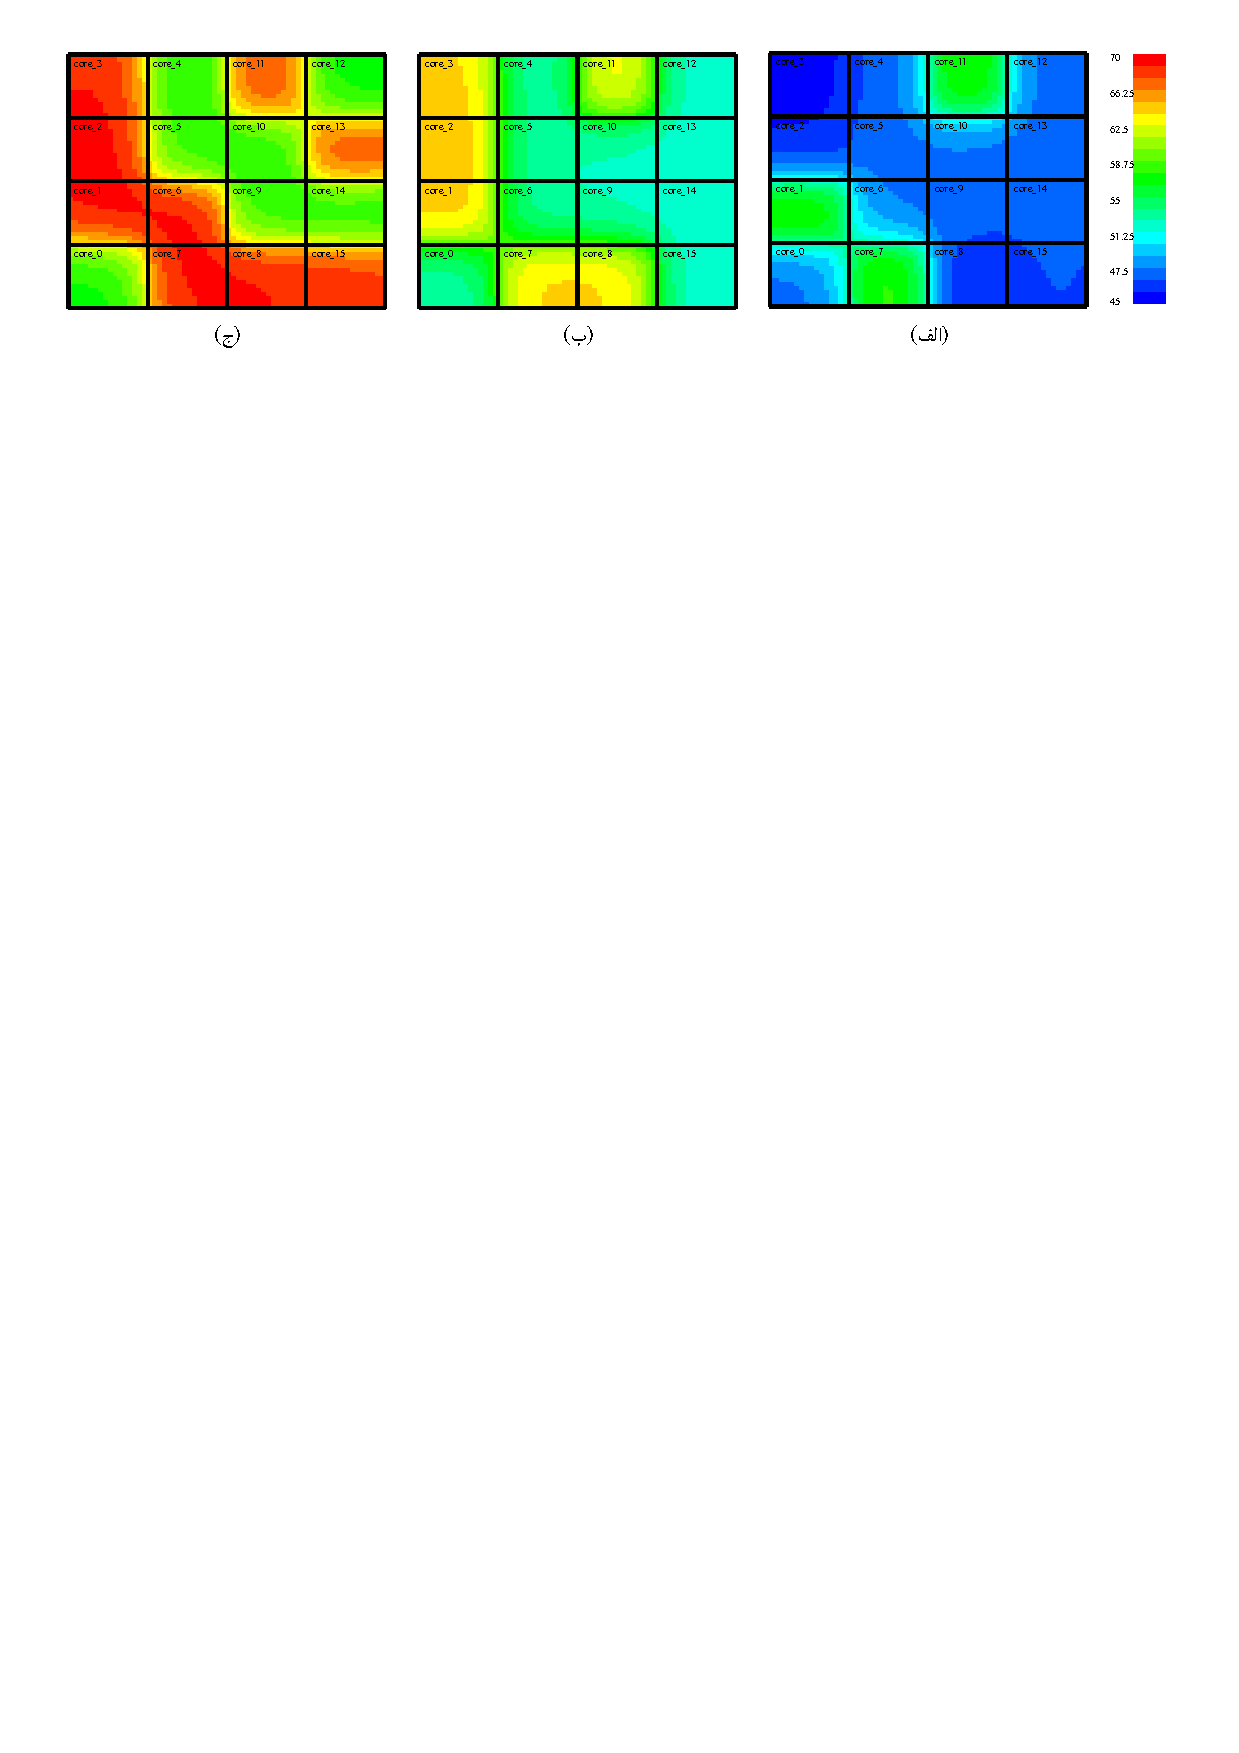
\includegraphics[scale=0.92]{images/ActiveCore.pdf}\\[0cm]
	\caption{بررسی تأثیر تعداد هسته‌های فعال بر دمای تراشه (الف) سه هسته‌ی فعال (ب) شش هسته‌ی فعال (ج) نه هسته‌ی فعال}
	\label{fig:ActiveCore}
\end{figure}


\section{نتایج ارزیابی}
در این بخش، رویکرد زمان‌بندی آگاه از دمای سطح تراشه و قابلیت اطمینان به کمک شبیه‌سازی مورد ارزیابی قرار می‌گیرد. در این پژوهش از شبیه‌سازهای 
\lr{gem5}\cite{binkert2011gem5}، \lr{McPAT}\cite{li2009mcpat}
و 
\lr{HotSpot}\cite{huang2006hotspot}
برای ارزیابی روش پیشنهادی استفاده می‌شود.
همچنین در شبیه‌سازی‌های انجام شده از بسته محک\efootnote{Benchmark}
\lr{MiBench} \cite{guthaus2001mibench}
برای مدل‌سازی کاربردهای واقعی استفاده شده است.\\






%\newline\newline

  \section{نتیجه‌گیری و کارهای آتی}
\label{sec:conclusion}
در این پژوهش سعی بر آن است که راه حلی برای مشکل افزایش دمای سطح تراشه که باعث بوجود آمدن مشکلاتی در زمینه‌ی رعایت قیود قابلیت اطمینان و بی‌درنگی سامانه‌های بحرانی-مختلط می‌شود، ارائه شود. همان‌گونه که دیده شد استفاده‌ی غیر اصولی از تمام هسته‌های یک تراشه با حداکثر فرکانس و ولتاژ، می‌تواند اثرات جانبی بسیاری برای سامانه داشته باشد. در این راستا یک روش آگاه از دمای سطح تراشه که قابلیت تحمل‌پذیری اشکال نیز داشته‌باشد می‌تواند کمک بسزایی به حفظ قابلیت اطمینان کند. در این پژوهش در ابتدا برای هر وظیفه حداقل ولتاژ و فرکانسی که قابلیت اطمینان را حفظ کنند، تعیین شد. در ادامه مفهومی به نام حداکثر هسته‌های فعال همزمان برای هر وظیفه بر اساس سقف توان مصرفی هر وظیفه با ولتاژ و فرکانسی که در مرحله‌ی قبل تعیین شد، بدست آمد و در ادامه زمان‌بندی نهایی بر اساس این فاکتور و روش تحمل‌پذیری اشکال چندپیمانه‌ای ارائه گردید. در کارهای آتی تلاش می‌شود تا کیفیت خدمات تا حد امکان افزایش یابد و مشکلات احتمالی روش پیشنهادی برطرف گردد و همچنین مقایسه‌ی کامل‌تری با کارهای موجود در این زمینه ارائه گردد. جدول\ref{tab:calender} زمان‌بندی کارهای صورت گرفته و آتی را نشان می‌دهد:


\begin{table}[h!]
 \centering
 \caption{مراحل انجام پروژه و زمان‌بندي آن}
\begin{tabular}{||c|c|c|c|c|c|c|c|c|
>{\columncolor[HTML]{EFEFEF}}c |c|c|c|c|c|c||}
\hline
\diagbox[height=15mm,width=46mm,dir=SW,innerrightsep=9mm]{\\زمان}{فعالیت}
%\slashbox[outerrightsep=-20pt]{فعالیت}{فعالیت}
%\diagbox{فعالیت}{فعالیت}

 &\rotatebox[origin=c]{90}{خرداد}
 &\rotatebox[origin=c]{90}{تیر}
 &\rotatebox[origin=c]{90}{مرداد}
 &\rotatebox[origin=c]{90}{شهریور}
 &\rotatebox[origin=c]{90}{مهر}
 &\rotatebox[origin=c]{90}{آبان}
 &\rotatebox[origin=c]{90}{آذر}
 &\rotatebox[origin=c]{90}{دی}
 &\rotatebox[origin=c]{90}{بهمن}
 &\rotatebox[origin=c]{90}{اسفند}
 &\rotatebox[origin=c]{90}{فروردین}
 &\rotatebox[origin=c]{90}{ اردیبهشت }
 &\rotatebox[origin=c]{90}{خرداد}
 &\rotatebox[origin=c]{90}{تیر}
 &\rotatebox[origin=c]{90}{مرداد}
\\ \hline
\begin{tabular}[c]{@{}c@{}}مطالعه و تحلیل کارهای پیشین\end{tabular}      & \checkmark & \checkmark & \checkmark & \checkmark &            &            &            &            &            &            &            &            &            &            &            \\ \hline
ارائه‌­ی روش پیشنهادی                                                         &            & \checkmark & \checkmark & \checkmark & \checkmark &            &            &            &            &            &            &            &            &            &            \\ \hline
پیاده­‌سازی روش پیشنهادی                                                      &            &            &            &            & \checkmark & \checkmark & \checkmark &            &            &            &            &            &            &            &            \\ \hline
ارزیابی کارهای پیشین                                                          &            &            &            &            & \checkmark & \checkmark & \checkmark & \checkmark &            &            &            &            &            &            &            \\ \hline
ارزیابی روش پیشنهادی                                                          &            &            &            &            &            & \checkmark & \checkmark & \checkmark & \checkmark &            &            &            &            &            &            \\ \hline
پیاده­‌سازی کارهای آتی و ارزیابی آن &            &            &            &            &            &            &            & \checkmark & \checkmark & \checkmark & \checkmark & \checkmark &            &            &            \\ \hline
نگارش پایان­‌نامه                                                           &            &            &            &            &            &            &            &            &            &            &            & \checkmark & \checkmark & \checkmark &            \\ \hline
آمادگی و دفاع از پایان­‌نامه                                                  &            &            &            &            &            &            &            &            &            &            &            &            &            &            & \checkmark \\ \hline
\end{tabular}
 \label{tab:calender}
\end{table}
 



%=========== Regular chapters ===============
%\cleardoublepage % terminates the current paragraph and page, the same way as a report document.
%\setlength{\headsep}{0in}
\setlatintextfont[Scale=0.7]{Times New Roman} 
\linespread{0.65} %line space
\renewcommand{\url}[1]{\underline{#1}}

%\bibliographystyle{IEEEtran}
%\bibliographystyle{is-unsrt}
\bibliographystyle{ieeetr-fa}
%\bibliographystyle{amsplain}


\newpage
\latin



\persian
%\setdigitfont[Scale=1]{B Nazanin}
%\settextfont[Scale=1.0]{B Nazanin}
\bibliography{resources}

\linespread{1} %line space

\newpage





\setlatintextfont[Scale=0.9]{Times New Roman} 
%\makeatletter
%\renewcommand{\@seccntformat}[1]{}
\makeatother
%\renewcommand*{\notesname}{ ‌}

\section*{واژه‌نامه}
{
	\renewcommand{\section}[2]{} % disable the automatic chapter
	\begin{RTL}
		\begin{multicols}{3}
			\theendnotes
		\end{multicols}
	\end{RTL}
}
\end{document}
